\documentclass{beamer}


% \usepackage{CJKnumb}\usepackage{beamerthemesplit}

\mode<article>
{
  \usepackage{beamerbasearticle}
  \usepackage{fullpage}
  \usepackage{hyperref}
}

%\usepackage{beamerthemesplit} 
%\usepackage{beamerthemeshadow}  
%\usepackage[width=2cm,dark,tab]{beamerthemesidebar}


% Setup appearance:

%\usetheme{Darmstadt}
\usefonttheme[onlylarge]{structurebold}
\setbeamerfont*{frametitle}{size=\normalsize,series=\bfseries}
\setbeamertemplate{navigation symbols}{}

\renewcommand\arraystretch{1.5}

% Standard packages

\usepackage[english]{babel}
%\usepackage[latin1]{inputenc}

\usepackage{epsf}
\usepackage{amsmath,amssymb}
\usepackage{graphicx}
\usepackage{tabularx}

% \usepackage[usenames,dvipsnames]{color}
\definecolor{shadow}{gray}{0.8}
\newcommand{\redc}[1]{{\color{red} #1}}
\newcommand{\bluec}[1]{{\color{blue} #1}}
\newcommand{\shadowc}[1]{{\color{shadow} #1}}
\definecolor{myyellow}{HTML}{FFB700}
\newcommand{\yellowc}[1]{{\color{myyellow} #1}}
\newcommand{\greenc}[1]{{\color{green} #1}}
\renewcommand{\v}[1]{\textbf{\textit{#1}}}
\renewcommand{\d}[1]{\textrm{#1}}


\usepackage{amsfonts}
\newcommand{\tickYes}{\checkmark}
\usepackage{pifont}
\newcommand{\tickNo}{\hspace{1pt}\ding{55}}

% \usetheme{Boadilla}
% \usetheme{Copenhagen}
% \usetheme{Madrid}
\usetheme{Singapore}


\begin{document}
%\title{Comparative atomistic and coarse-grained study of water: Simulation details vs. Simulation feasibility}
%\title[Optimizing SPME]{Optimizing Working Parameters of the Smooth Particle Mesh Ewald Algorithm}
\title[]{Accurate and Efficient Calculation of the Non-bonded Particle Interactions}
%
\author{Han Wang}
\institute[FUB] {
  Institut f\"ur Mathematik, Freie Universit\"at Berlin, Berlin\\
  School of Mathematical Sciences, Peking University, Beijing\\
\vskip 0.4cm
Joint with: Florian Dommert, Christian Holm, Pingwen Zhang}
\date[27 Oct 2011]{27 Oct 2011}
\frame{\titlepage}


\begin{frame}{Molecular dynamics simulation}
  \begin{itemize}\itemsep -10pt
  \item<1-> Molecular dynamics simulation:
    \bluec{
      \begin{align*}
        m_i \frac{\d d^2\v r_i}{\d dt^2} = \v F_i, \quad i = 1, 2, \cdots, N
      \end{align*}
    }
  \item<2-> Pairwise interaction:
    \bluec{
      \begin{align*}
        \v F_i = \sum_{j}\, \v f(\v r_i - \v r_j)
      \end{align*}}
  \item<3-> Periodic boundary condition:
    \bluec{
      \begin{align*}
        \v F_i = \sum_{\v n}^\ast\sum_{j}\, \v f(\v r_i - \v r_j + \v n)
      \end{align*}}
  \end{itemize}
\end{frame}

\begin{frame}{Fast algorithms}
  \begin{itemize}
  \item<1-> Naive computation of pairwise interaction costs \redc{$\mathcal O(N^2)$}
  \item<2-> Fast algorithm:
    \begin{figure}
      \centering 
      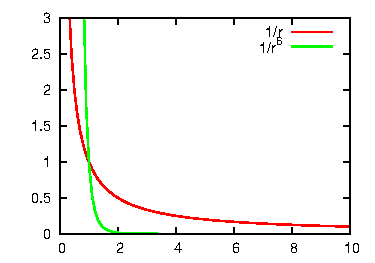
\includegraphics[width=0.5\textwidth]{figs/long-range/decay.pdf}
    \end{figure}
    \begin{itemize}
    \item<3-> Short-range interaction: \bluec{$1/r^6$}\quad Cut-off method \redc{$\mathcal O(N)$}
    \item<4-> Long-range interaction: \bluec{$1/r$}\quad \ \ SPME method \redc{$\mathcal O(N \log N)$}
    \end{itemize}
  \end{itemize}
\end{frame}

\begin{frame}{Error of fast algorithms}
  \begin{figure}
    \centering
    \begin{minipage}[c]{.48\textwidth}
      \centering
      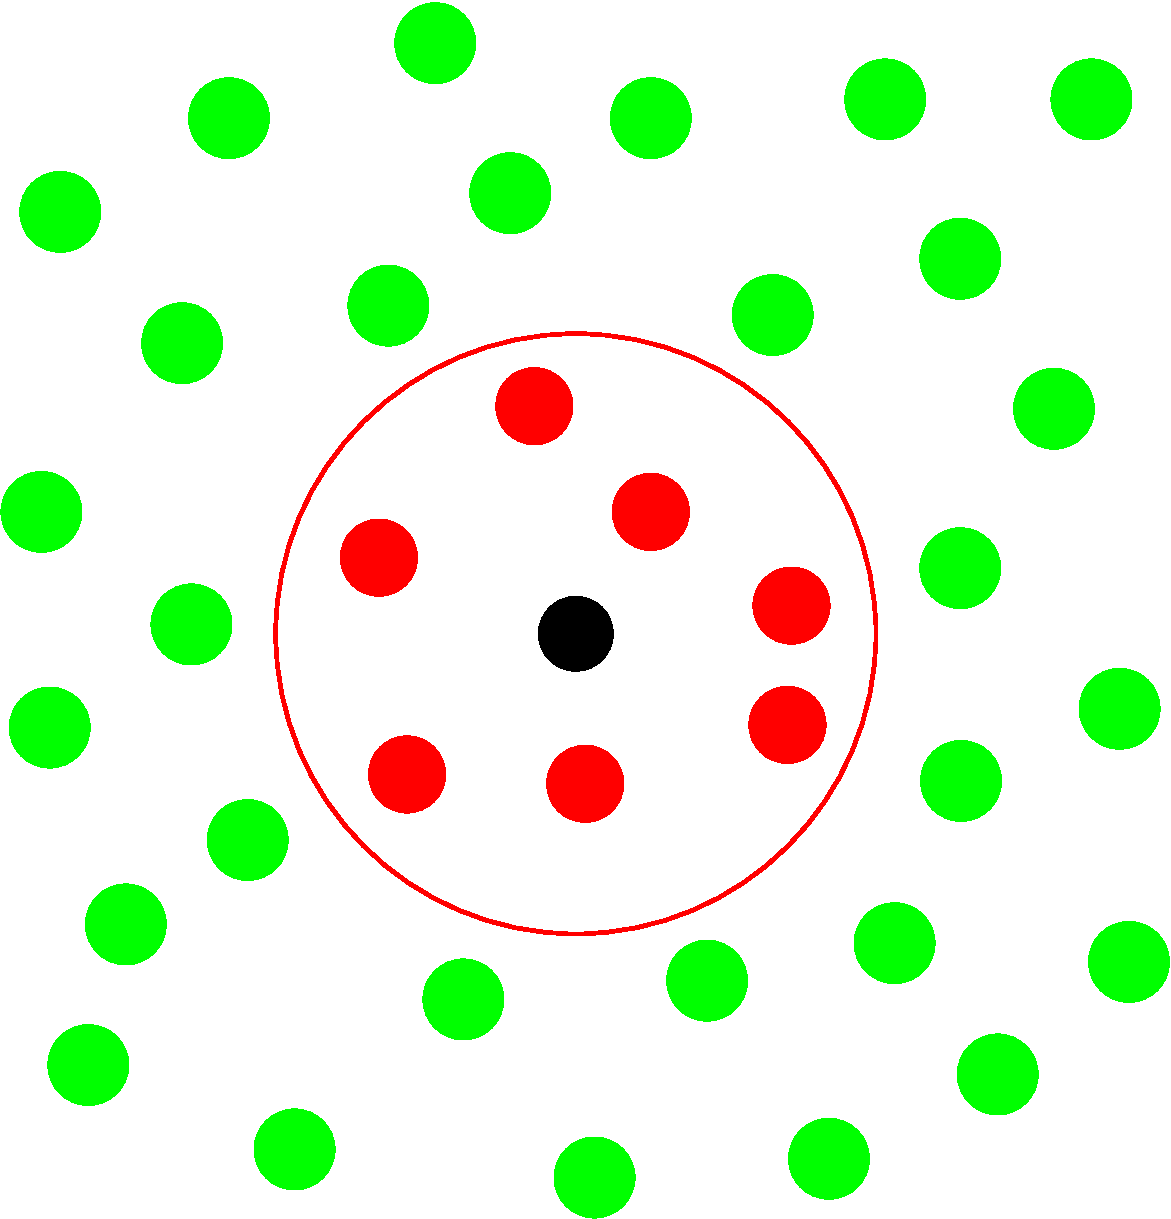
\includegraphics[width=0.7\textwidth]{figs/short-range//simple-cutoff.pdf}      
    \end{minipage}
    \begin{minipage}[c]{.50\textwidth}
      \centering
      \vskip .5cm
      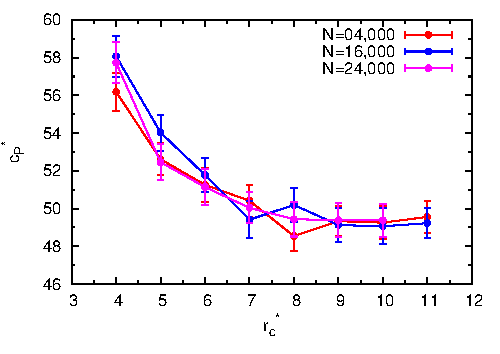
\includegraphics[width=1.0\textwidth]{figs/simple-cut-conv/natom-rcut-c.pdf}
    \end{minipage}
    \end{figure}
  \begin{itemize}
  \item<1-> However, there is \redc{NO} free lunch... Error of force.
  \item<2-> Mostly used $r_c$: 2.5 -- 4.0 $\sigma$. \redc{Convergence check} required.
  \item<3-> How cut-off method works. Cost \redc{$\mathcal O(r_c^3)$}.
  \item<4-> Quantitatively: the \redc{error estimate}.
  \end{itemize}
\end{frame}

\begin{frame}{Definition of force error}
  \begin{itemize}
  \item<1->   The difference between exact force and computed force by fast algorithms:
  \bluec{
    \begin{align*}
      \Delta\v F(\v r) = \v F(\v r) - \tilde{\v F}(\v r),
    \end{align*}
  }
  which is called \redc{error force}.
  \vskip .5cm
  \item<2-> error \bluec{$\mathcal E$}: the root mean square (RMS) of the error force:
  \redc{
    \begin{align*}
      \mathcal E =\sqrt{ \langle\vert\Delta\v F(\v r)\vert^2\rangle}
    \end{align*}
    }
  \end{itemize}
\end{frame}

\begin{frame}{Overview of the error estimates}
  \begin{itemize}
  \vfill
  \item<1->   Conditions for the error estimate:
  \begin{enumerate}\itemsep 3pt
  \item \redc{Homogeneity}.
  \item Particles are \redc{uncorrelated}.
  \end{enumerate}
  \vfill
\item<2->   Current error estimates:
  \begin{table}
    \centering
    \begin{tabular*}{0.85\textwidth}{l@{\extracolsep{\fill}}ll}\hline\hline
      Conditions & Short-range & Long-range \\\hline
      1+2 & \bluec{\tickYes\quad$\mathcal O(1)$}  & \redc{\tickYes\quad$\mathcal O(1)$} \\
      2   & \redc{\tickYes\quad$\mathcal O(N\log N)$} & \redc{\tickYes\quad$\mathcal O(N\log N)$} \\
      none& \redc{\tickNo\quad$\mathcal O(N^2\log N)$} & \redc{\tickNo\quad$\mathcal O(N^2\log N)$} \\\hline\hline
    \end{tabular*}
  \end{table}
  \vfill
  \end{itemize}
\end{frame}

\begin{frame}{Short-range, homogeneous, uncorrelated}
  \begin{enumerate}\itemsep 3pt
  \item {Homogeneity}.
  \item Particles are {uncorrelated}.
  \end{enumerate}
    \begin{table}
    \centering
    \begin{tabular*}{0.85\textwidth}{l@{\extracolsep{\fill}}ll}\hline\hline
      Conditions & Short-range & Long-range \\\hline
      1+2 & \bluec{\tickYes\quad$\mathcal O(1)$}  & \shadowc{\tickYes\quad$\mathcal O(1)$} \\
      2   & \shadowc{\tickYes\quad$\mathcal O(N\log N)$} & \shadowc{\tickYes\quad$\mathcal O(N\log N)$} \\
      none& \shadowc{\tickNo\quad$\mathcal O(N^2\log N)$} & \shadowc{\tickNo\quad$\mathcal O(N^2\log N)$} \\\hline\hline
    \end{tabular*}
  \end{table}
\end{frame}

\begin{frame}{Short-range, homogeneous, uncorrelated}
  \begin{itemize}\itemsep -10pt
    \vfill
  \item<1-> Error estimate:
    \bluec{
      \begin{align*}
        \mathcal E^2(r_c) = 4\pi\rho\int_{r_c}^\infty r^2[u'(r)]^2 \,\d dr,
      \end{align*}}
    where \bluec{$u(r)$} is the pairwise interaction potential.
    \vfill
    \vskip 1.cm
  \item<2-> Homogeneity $\Rightarrow$ \bluec{$\langle\Delta\v F\rangle = 0$}
    \bluec{
      \begin{align*}
        \mathcal E^2 = \textrm{Var}(\Delta\v F)
      \end{align*}
    }
    \vfill
  \end{itemize}
\end{frame}

\begin{frame}{Short-range, inhomogeneous, correlated}
  \begin{enumerate}\itemsep 3pt
  \item {Homogeneity}.
  \item Particles are {uncorrelated}.
  \end{enumerate}
    \begin{table}
    \centering
    \begin{tabular*}{0.85\textwidth}{l@{\extracolsep{\fill}}ll}\hline\hline
      Conditions & Short-range & Long-range \\\hline
      1+2 & \shadowc{\tickYes\quad$\mathcal O(1)$}  & \shadowc{\tickYes\quad$\mathcal O(1)$} \\
      2   & \redc{\tickYes\quad$\mathcal O(N\log N)$} & \shadowc{\tickYes\quad$\mathcal O(N\log N)$} \\
      none& \redc{\tickNo\quad$\mathcal O(N^2\log N)$} & \shadowc{\tickNo\quad$\mathcal O(N^2\log N)$} \\\hline\hline
    \end{tabular*}
  \end{table}
\end{frame}

\begin{frame}{Short-range, inhomogeneous, correlated}
  \begin{itemize}\itemsep 10pt
  \item<1-> Example system:
    \begin{figure}
      \centering
      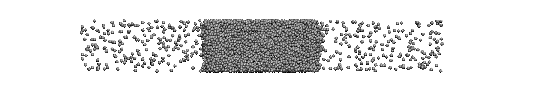
\includegraphics[width=0.9\textwidth]{figs/t0.85-n16000-rc07.5uni/confout-02.eps}
    \end{figure}
  \item<2-> Equilibrium densities:
    \begin{figure}
    \centering
    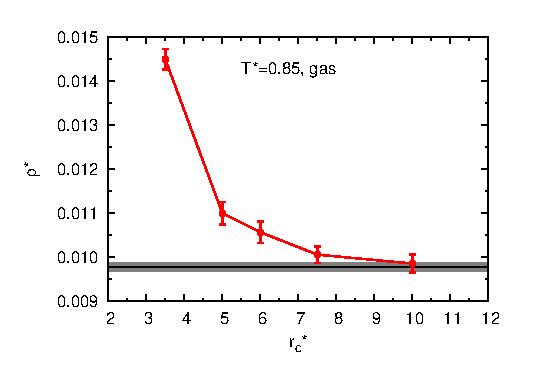
\includegraphics[width=0.49\textwidth]{figs/converge.new/t0p85-gas-1.eps} 
    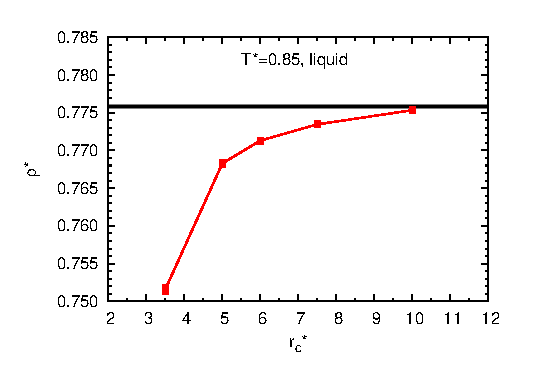
\includegraphics[width=0.49\textwidth]{figs/converge.new/t0p85-liquid-1.eps} 
  \end{figure}  
  \end{itemize}
\end{frame}

\begin{frame}{Short-range, inhomogeneous, correlated}
  \begin{itemize}\itemsep -10pt
  \item<1->   The mean error force is
  \bluec{
    \begin{align*}
      \langle\Delta\v F(\v r)\rangle
      =
      \int_{\mathbb R^3}\v f^c(\v r - \v r')\rho(\v r')\,\d d\v r'
      \neq 0
    \end{align*}
  }
  \vskip -10cm
\item<2->   The error:
  \bluec{
    \begin{align*} \nonumber
      \langle\vert\Delta\v F(\v r)\vert^2\rangle
      = 
      \redc{\mathcal E^2_{\textrm{homo}}(\v r)} +
      % \langle\Delta\v F(\v r)\,\rangle^2 +
      \redc{\mathcal E^2_{\textrm{inhomo}}(\v r)} +
      \redc{\mathcal E_{\textrm{correlation}}(\v r)}.
    \end{align*}
  }
  with\bluec{
  \begin{align*}
    \redc{\mathcal E^2_{\textrm{homo}}(\v r)}
    = &\,
    \int_{\mathbb R^3}\vert\v f^c(\v r - \v r')\vert^2\rho(\v r')\,\d d\v r'  \\
    \redc{\mathcal E^2_{\textrm{inhomo}}(\v r)}
    = &\,
    \bigg[\int_{\mathbb R^3}\v f^c(\v r - \v r')\rho(\v r')\,\d d\v r'\,\bigg]^2
    \redc{ = \langle\Delta\v F(\v r)\,\rangle^2}
    \\
    \redc{\mathcal E_{\textrm{correlation}}(\v r)}
    =&\,
    \int_{\mathbb R^3\times\mathbb R^3}\v f^c(\v r - \v r')\cdot\v f^c(\v r - \v r'')\,C(\v r', \v r'')\,\d d\v r'\d d\v r''
  \end{align*}}
  \end{itemize}
\end{frame}


\begin{frame}{Short-range, inhomogeneous, correlated}{Notations}
  \vfill
  \bluec{$\rho(\v r)$} is the number density of the system.
  \vfill  
  The complementary of the cut-offed force is:
  \bluec{
    \begin{align*}
      \v f^c(\v r) =
      \left\{
        \begin{array}{ll}
          0, & \vert\v r\vert\leq r_c; \\
          \v f(\v r), & \vert\v r\vert > r_c.
        \end{array}
      \right.
    \end{align*}}  
  \vfill  
  The Correlation function:
  \bluec{
    \begin{align*}
      C (\v r', \v r'') = [\,\rho(\v r', \v r'') -  \rho(\v r')\rho(\v r'')\,]
    \end{align*}}
  \vfill  
\end{frame}


\begin{frame}{Liquid-vapor equilibrium}
  \begin{figure}
    \centering
    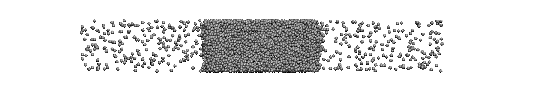
\includegraphics[scale=1]{figs/t0.85-n16000-rc07.5uni/confout-02.eps}\\
    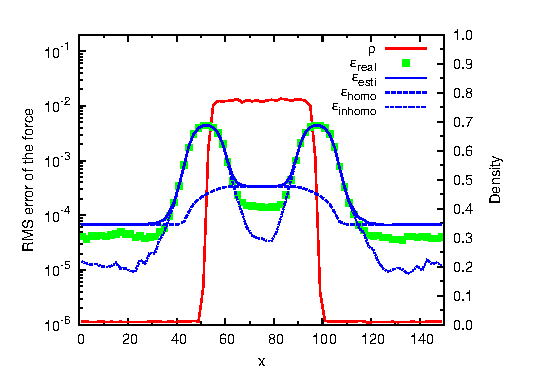
\includegraphics[]{figs/t0.85-n16000-rc07.5uni/error-uniform.eps}
  \end{figure}
\end{frame}

\begin{frame}{Adaptive cut-off radius}
  \begin{figure}
    \centering
    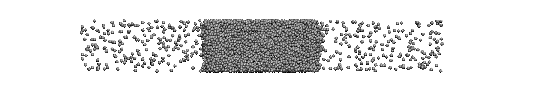
\includegraphics[scale=1]{figs/t0.85-n16000-rc07.5uni/confout-02.eps}\\
    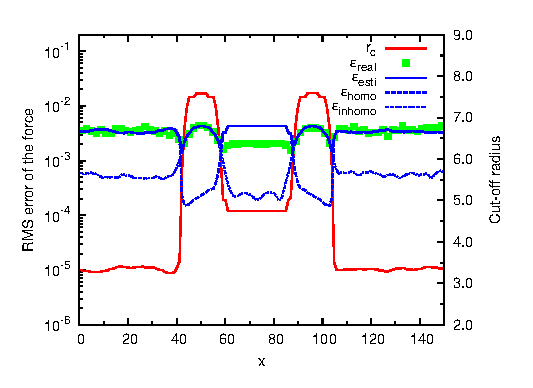
\includegraphics[]{figs/t0.85-n16000-adapt-e0.0045-extend/rcut-and-error.eps}
  \end{figure}
\end{frame}

\begin{frame}{Long-range force correction}
  \begin{itemize}\itemsep -10pt
  \item<1->   Force correction:
  \bluec{
\begin{align*}
  \v F_{\textrm{corr}}(\v r) =
  \tilde{\v F}(\v r) +
  \redc{\langle\Delta\v F(\v r)\rangle}.
\end{align*}}
\item<2->   The mean of
  the corrected error force vanishes:
  \bluec{
\begin{align*}
  \langle\Delta\v F_{\textrm{corr}}(\v r)\rangle
   =
  \big\langle\,
  \v F(\v r) - \tilde{\v F}(\v r) - \langle\Delta\v F(\v r)\rangle\,
  \big\rangle = 0.
\end{align*}}
\item<3-> The mean square error is given by
\bluec{
\begin{align*} \nonumber
  \langle\vert\Delta\v F_{\textrm{corr}}(\v r)\vert^2\rangle
   =
   \redc{\mathcal E^2_{\textrm{homo}}(\v r)} +
   \redc{\mathcal E_{\textrm{correlation}}(\v r)}.
\end{align*}}
which contains \redc{NO} inhomogeneous part.
  \end{itemize}
\end{frame}

\begin{frame}{Long-range force correction}
  \begin{figure}
    \centering
    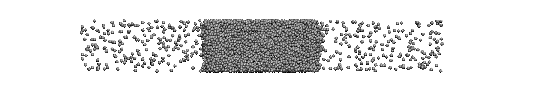
\includegraphics[scale=1]{figs/t0.85-n16000-rc07.5uni/confout-02.eps}\\
    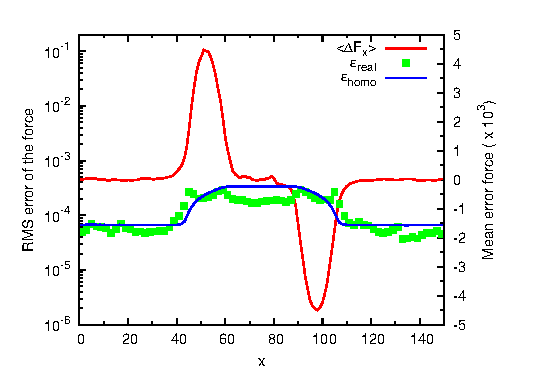
\includegraphics[]{figs/t0.85-n16000-fcorr-rc07.5-feq0200/fcorr-and-error.eps}
  \end{figure}
\end{frame}

\renewcommand\arraystretch{1.1}
\begin{frame}{Accuracy and efficiency}
  \begin{table}
  \centering
  \begin{tabular*}{0.8\textwidth}{c|@{\extracolsep{\fill}}lcc}\hline\hline
    $r^\ast_{c}$ & \textrm{method} & $\max\mathcal E^\ast$ & Cost($\times 10^{-6}$) \\ \hline
     &\textrm{uniform} & $8.6\times 10^{-2}$ & 2.9 \\
 3.5 &\textrm{adaptive} & $8.6\times 10^{-2}$ & 1.9 \\
     &\textrm{force corr} & $1.4\times 10^{-2}$ & 3.1 \\\cline{1-4}
     &\textrm{uniform} & $2.2\times 10^{-2}$ & 7.8 \\
 5.0 &\textrm{adaptive} & $2.2\times 10^{-2}$ & 4.5 \\
     &\textrm{force corr} & $1.9\times 10^{-3}$ & 7.9 \\\cline{1-4}
 6.0 &\textrm{uniform} & $1.1\times 10^{-2}$ & 13 \\\cline{1-4}
     &\textrm{uniform} & $4.5\times 10^{-3}$ & 24 \\
 7.5 &\textrm{adaptive} & $4.3\times 10^{-3}$ & 12 \\
     &\textrm{force corr} & $2.3\times 10^{-4}$ & 24 \\\cline{1-4}
     &\textrm{uniform} & $1.4\times 10^{-3}$ & 53 \\
10.0 &\textrm{adaptive} & $1.4\times 10^{-3}$ & 26 \\
     &\textrm{force corr} & $5.3\times 10^{-5}$ & 53 \\ \hline\hline
  \end{tabular*}
\end{table}
\end{frame}
\renewcommand\arraystretch{1.5}


\begin{frame}{Equilibrium gas density}
  \begin{figure}
    \centering
    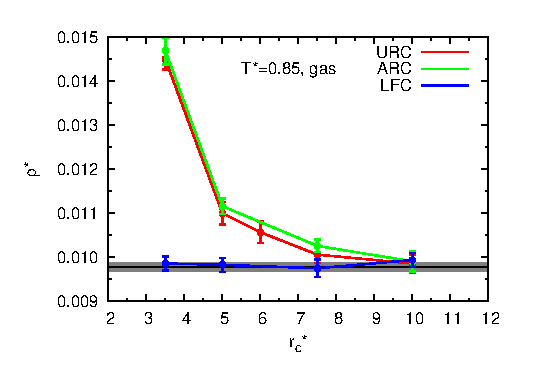
\includegraphics[]{figs/converge.new/t0p85-gas.eps} 
  \end{figure}
  URC: uniform cut-off, ARC: adaptive cut-off, LFC: long-range force correction.
\end{frame}

\begin{frame}{Equilibrium liquid density}
  \begin{figure}
    \centering
    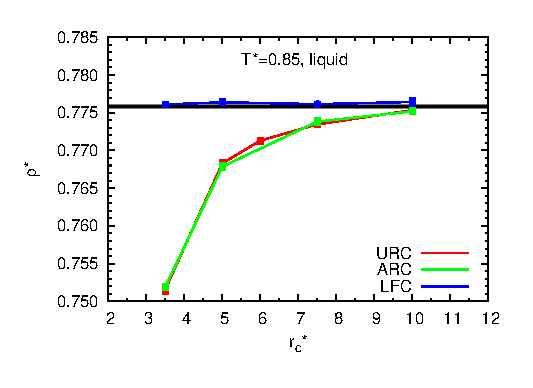
\includegraphics[]{figs/converge.new/t0p85-liquid.eps} 
  \end{figure}
  URC: uniform cut-off, ARC: adaptive cut-off, LFC: long-range force correction.
\end{frame}


\begin{frame}{Conclusion}
  \centerline{\redc{The inhomogeneity error is bad}}.
\end{frame}

\begin{frame}{Electrostatic interaction and Ewald summation}
  \begin{itemize}
  \item<1->   Electrostatic interaction:
  \begin{equation*}\bluec{
    U_{\textrm{ele}} = \frac12 \sum^\ast_{n}\sum_{i,j}\frac{q_i q_j}{\vert \v r_{ij} + \v n\vert}}
  \end{equation*}
\item <2->
  Ewald summation (1921) splits the
  energy into three parts
  \bluec{
  \begin {align*}
    U_{\textrm{ele}} &=  U_{\textrm{dir}} + U_{\textrm{rec}}+ U_{\textrm{corr}}\\
    U_{\textrm{dir}} & = \frac12 \sum^{\ast}_{\v n}
    \sum_{i,j = 1}^{N} \frac{q_iq_j\, \redc{\textrm{erfc}(\beta \vert\v{r}_{ij} + \v{n}\vert)}}
    {\vert\v{r}_{ij} + \v{n}\vert} \\ \label{Erec-ewald}
    U_{\textrm{rec}} & = \frac1{2\pi V} \sum_{\v m \neq 0}
    \frac{\redc{\exp(-\pi^2\v m^2 / \beta^2)}}{\v m^2} S(\v m) S(-\v m) \\
    U_{\textrm{corr}}& = -\frac\beta{\sqrt \pi} \sum_{i=1}^N q_i^2
  \end {align*}}
  \end{itemize}
\end{frame}


\begin{frame}{Smooth Particle Mesh Ewald Method (SPME)}
  \begin{itemize}\itemsep -5pt
  \item<1-> The structure factor \bluec{$S(\v m)$} is
    defined by \bluec{
      \begin{equation*}\label{sm1}
        S(\v m) = \sum_{j=1}^N q_j \exp (2 \pi i \v m \cdot \v r_j),
      \end{equation*}}
  \item<2-> Optimal computational cost\footnote{
    \bluec{J. Perram, H. Petersen and S. De Leeuw, Mol. Phys. \textbf{65}, 875 (1988).}}: \redc{$\mathcal O(N^{1.5})$}.
    \vskip .5cm
  \item<3-> \redc{SPME}\footnote{
    \bluec{U. Essmann, \textit{et. al.}, J. Chem. Phys. \textbf{103}, 8577 (1995).}}: interpolate \bluec{$S(\v m)$} on grid, then FFT.
    The computational cost is 
  \begin{align*}
    \begin{tabular}[t]{c}
      \redc{$\mathcal O(N)$}\\
      {direct}
    \end{tabular}
    +
    \begin{tabular}[t]{c}
      \redc{$\mathcal O(N)$}\\
      {interpolation}
    \end{tabular}
    +
    \begin{tabular}[t]{c}
      \redc{$\mathcal O(N\log N)$}\\
      {FFTs}
    \end{tabular}
    =
    \begin{tabular}[t]{c}
      \redc{$\mathcal O(N\log N)$}\\
      {total cost}
    \end{tabular}
    \end{align*}
  \end{itemize}
\end{frame}

\begin{frame}{Smooth Particle Mesh Ewald Method (SPME)}{Working parameters}
  \vfill
  To use SPME method, one should provide the following parameters.
  \vfill
  \begin{itemize}
    \item \redc{$\beta$} \quad The controlling parameter.
    \item \redc{$r_c$} \quad The direct space cut-off radius.
    \item \redc{$\v K$} \quad The reciprocal space cut-off. The number of FFT grid points.
    \item \redc{$n$} \quad The order of cardinal B-spline interpolation.
  \end{itemize}
  \vfill An arbitrary combination may lead to \redc{totally wrong
    results}. \vfill
\end{frame}

\begin{frame}{SPME, homogeneous, uncorrelated}
  \begin{enumerate}\itemsep 3pt
  \item {Homogeneity}.
  \item Particles are {uncorrelated}.
  \end{enumerate}
    \begin{table}
    \centering
    \begin{tabular*}{0.85\textwidth}{l@{\extracolsep{\fill}}ll}\hline\hline
      Conditions & Short-range & Long-range \\\hline
      1+2 & \shadowc{\tickYes\quad$\mathcal O(1)$}  & \redc{\tickYes\quad$\mathcal O(1)$} \\
      2   & \shadowc{\tickYes\quad$\mathcal O(N\log N)$} & \shadowc{\tickYes\quad$\mathcal O(N\log N)$} \\
      none& \shadowc{\tickNo\quad$\mathcal O(N^2\log N)$} & \shadowc{\tickNo\quad$\mathcal O(N^2\log N)$} \\\hline\hline
    \end{tabular*}
  \end{table}
\end{frame}

\begin{frame}{SPME, homogeneous, uncorrelated}
  \begin{figure}
  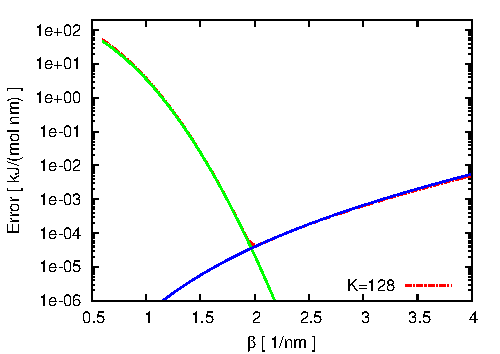
\includegraphics[width=0.7\textwidth]{figs/long-range//bspline-order6.pdf}
\end{figure}
  The error estimate\footnote{
    \bluec{H. Wang, F. Dommert and C. Holm, J. Chem. Phys. \textbf{133}, 034117 (2010).}}
  is available in MD package Gromacs \redc{now}.
\end{frame}

\begin{frame}{SPME, homogeneous, uncorrelated}{Parameter tuning}
  The parameter tuning is a constrained optimization problem:\footnote{
    \bluec{H. Wang, F. Dommert and C. Holm, J. Chem. Phys. \textbf{133}, 034117 (2010).}}
  \bluec{
  \begin{align*} 
    \min\quad &  T (r_c, \v K, n, \beta),\\
    \textrm{\textbf{s.t.}}\quad & \mathcal E (r_c, \v K, n, \beta) = \mathcal E_{\textrm{C}}
  \end{align*}}
Available in MD package Gromacs \bluec{soon}.
\end{frame}

\begin{frame}{Ewald summation, inhomogeneous, correlated}
  \begin{enumerate}\itemsep 3pt
  \item {Homogeneity}.
  \item Particles are {uncorrelated}.
  \end{enumerate}
  \begin{table}
    \centering
    \begin{tabular*}{0.85\textwidth}{l@{\extracolsep{\fill}}ll}\hline\hline
      Conditions & Short-range & Long-range \\\hline
      1+2 & \shadowc{\tickYes\quad$\mathcal O(1)$}  & \shadowc{\tickYes\quad$\mathcal O(1)$} \\
      2   & \shadowc{\tickYes\quad$\mathcal O(N\log N)$} & \redc{\tickYes\quad$\mathcal O(N\log N)$} \\
      none& \shadowc{\tickNo\quad$\mathcal O(N^2\log N)$} & \redc{\tickNo\quad$\mathcal O(N^2\log N)$} \\\hline\hline
    \end{tabular*}
  \end{table}
\end{frame}

\begin{frame}{Ewald summation, inhomogeneous, correlated}
  \begin{itemize}\itemsep -10pt
  \item<1->   Recall the reciprocal part error:
  \bluec{
    \begin{align*}
      \Delta U_{\textrm{rec}} & = \frac1{2\pi V}    
      \sum_{
        \begin{subarray}{c}
          \vert m_\alpha\vert \geq K_\alpha/2\\
          \v m\neq 0
        \end{subarray}}
      \frac{{\exp(-\pi^2\v m^2 / \beta^2)}}{\v m^2} \,S(\v m) \,S(-\v m) 
    \end{align*}}
\item<2->   The mean error force is:
  \bluec{
    \begin{align*}
      \big\langle
      \Delta \v F(\v r)
      \big\rangle
      =
      q \int \v G_c(\v r - \v r') \,\rho_q(\v r')\,\d d\v r',
    \end{align*}}
\item<3->   where
  \bluec{
    \begin{align*}
      \v G_c(\v r) =
      \sum_{
        \begin{subarray}{c}
          \vert m_\alpha\vert \geq K_\alpha/2\\
          \v m\neq 0
        \end{subarray}}
      4\pi\v mi\frac{\exp(-\pi^2 \v m^2 / \beta^2)}{2\pi V \v m^2}
      e^{2\pi i\v m\cdot\v r}\,
    \end{align*}
  }
  \end{itemize}
\end{frame}


\begin{frame}{Ewald summation, inhomogeneous, correlated}
  \begin{itemize}\itemsep 15pt
  \item<1-> \bluec{$\rho_q(\v r)$} is the charge density:
    \begin{align*}
      \bluec{  \rho_q(\v r) = 
        \bigg\langle
        \sum_{j = 1}^N
        q_j\delta(\v r - \v r_j)
        \bigg\rangle
      }
    \end{align*}
    Varnishes if the system is \redc{locally neutral}.
  \item<2-> The Fourier modes of mean error force:
    \bluec{
      \begin{align*}
        \langle\Delta\v F\rangle^\wedge(\v k) =
        \left\{
          \begin{aligned}[c]
            & \quad 0, & & \textrm{if}\ \vert k_\alpha\vert\leq K_\alpha/2 \\
            & 4\pi\v ki\frac{\exp(-\pi^2 \v k^2 / \beta^2)}{2\pi V \v k^2}\times\hat\rho_q(\v k),
            & & \textrm{Otherwise}.
          \end{aligned}
        \right.
      \end{align*}}
    small if density is \redc{smooth}.
  \end{itemize}
\end{frame}



\begin{frame}{Ewald summation, inhomogeneous, correlated}
  The force error:
    \bluec{
    \begin{align*} \nonumber
      \langle\vert\Delta\v F(\v r)\vert^2\rangle
      = 
      \redc{\mathcal E^2_{\textrm{homo}}(\v r)} +
      % \langle\Delta\v F(\v r)\,\rangle^2 +
      \redc{\mathcal E^2_{\textrm{inhomo}}(\v r)} +
      \redc{\mathcal E_{\textrm{correlation}}(\v r)}.
    \end{align*}
  }
  with\bluec{
    \begin{align*}
      \redc{\mathcal E^2_{\textrm{homo}}(\v r)}
      = &\,
      q^2\int_{\mathbb R^3}\vert\v G_c(\v r - \v r')\vert^2\rho_{q^2}(\v r')\,\d d\v r'  \\
      \redc{\mathcal E^2_{\textrm{inhomo}}(\v r)}
      = &\,
      q^2 \bigg[\int_{\mathbb R^3}\v G_c(\v r - \v r')\,\rho_q(\v r')\,\d d\v r'\,\bigg]^2
      \redc{ = \langle\Delta\v F(\v r)\,\rangle^2}\\
          \redc{\mathcal E_{\textrm{correlation}}(\v r)}
    =&\,
    q^2\int_{\mathbb R^3\times\mathbb R^3}\v G_c(\v r - \v r')\cdot\v G_c(\v r - \v r'')\,C_{q^2}(\v r', \v r'')\,\d d\v r'\d d\v r''
    \end{align*}}
  where
    \begin{align*}
      \bluec{  \rho_{q^2}(\v r) = 
        \bigg\langle
        \sum_{j = 1}^N
        q^2_j\delta(\v r - \v r_j)
        \bigg\rangle
      }
    \end{align*}
\end{frame}


\begin{frame}{SPME, inhomogeneous, correlated}
  \centerline{
    The \redc{same}. With different convolution kernels.}
\end{frame}

\begin{frame}{Summary}
  \begin{itemize}\itemsep -10pt
  \item<1-> The error estimate in an inhomogeneous and correlated system is:
    \bluec{
      \begin{align*} \nonumber
        \langle\vert\Delta\v F(\v r)\vert^2\rangle
        = 
        \redc{\mathcal E^2_{\textrm{homo}}(\v r)} +
        % \langle\Delta\v F(\v r)\,\rangle^2 +
        \redc{\mathcal E^2_{\textrm{inhomo}}(\v r)} +
        \redc{\mathcal E_{\textrm{correlation}}(\v r)}.
      \end{align*}
    }
  \item<2-> Inhomogeneity error $ \bluec{\mathcal E^2_{\textrm{inhomo}}(\v
      r) = }\redc{\langle\Delta\v F(\v r)\rangle^2}$ is bad...
    \vfill
  \item<3-> For short-range, the error estimate enable:
    \begin{itemize}
    \item \redc{adaptive cut-off simulation} 
    \item \redc{long-range force correction}.
    \end{itemize}
    \vfill
  \item<4-> Homogeneity error estimate for SPME: \redc{parameter tuning}.
    \vfill
  \item<5-> The inhomogeneity error estimate for long-range interaction:
    we are \redc{safe} in most simulations.
    \vfill
  \end{itemize}
\end{frame}

% \begin{frame}{Other research interests}
%   \begin{itemize}
%   \item 
%   \end{itemize}
% \end{frame}

\begin{frame}
  \vfill
  \centerline{ \Huge
    Thanks!  }
  \vfill
  \bluec{
    \begin{align*} \nonumber
      \langle\vert\Delta\v F(\v r)\vert^2\rangle
      = 
      \redc{\mathcal E^2_{\textrm{homo}}(\v r)} +
      % \langle\Delta\v F(\v r)\,\rangle^2 +
      \redc{\mathcal E^2_{\textrm{inhomo}}(\v r)} +
      \redc{\mathcal E_{\textrm{correlation}}(\v r)}.
    \end{align*}
  }
\end{frame}


\end{document}
